In order to use the weak formulation, \texttt{FastFEM} needs to know how to integrate functions on a given mesh. Each element type specifies both the shape functions and the algorithm used to integrate a function on that element. For example, the mass matrix entries (\ref{eqn:mass_matrix}) on two different element types are:

\begin{itemize}
\item For linear triangular elements with shape functions $\{\phi_1,\phi_2,\phi_3\}$ having the Kronecker delta property for each vertex ($\phi_i(v_j) = \delta_{ij}$ for vertices $v_1,v_2,v_3$), the analytical solution to the integral is known, since the shape functions are linear.

\item Spectral elements, a technique used in fluid dynamics (Patera 1984)\supercite{Patera1984} and other continuum mechanical fields, have shape functions $\phi_{i_1,i_2}(F(x,y)) = L_{i_1}(x)L_{i_2}(y)$ for Lagrange interpolation polynomials $L_i$ based on GLL (Gauss-Lobatto-Legendre) quadrature\supercite{Quarteroni2007}, where $F$ denotes the coordinate transform from a reference space $[-1,1]^2$ to the element in the mesh's space. Integration is done using GLL quadrature in order to produce a diagonal mass matrix, so the integral is computed
\begin{equation}
\begin{aligned}
    \int_{\Omega_{SE}} \phi_{i_1,i_2}\phi_{j_1,j_2} ~dV = \int_{\Omega_{SE}} L_{i_1}(x)L_{i_2}(y)L_{j_1}(x)L_{j_2}(y) ~dV \\
    \approx \sum_{k_1,k_2=0}^N \alpha_{k_1}\alpha_{k_2} J(F(t_{k_1},t_{k_2}))L_{i_1}(t_{k_1})L_{i_2}(t_{k_2})L_{j_1}(t_{k_1})L_{j_2}(t_{k_2}) \\
    = \alpha_{i_1}\alpha_{i_2}J(F(t_{k_1},t_{k_2}))\delta_{i_1,j_1}\delta_{i_2,j_2}
\end{aligned},
\label{eqn:spectral_mass_matrix}
\end{equation}
where $J = \rho|\det DF|$ is the Jacobian with some scaling parameter $\rho$, which may vary in space. This is relevant for PDEs with a varying mass term.
\end{itemize}


\subsubsection{Elements} \label{sec:elem_field:elements}
To employ the different behaviors, elements inherit from a superclass that with abstract methods for each integral. For $H^1$ elements in 2D, these are


\begin{verbatim}
element.integrate_field(position_field, field, jacobian_scale)
\end{verbatim}

\begin{equation}
\int_{\Omega_E} f~dV
\label{eqn:element_integrate_field}
\end{equation}

\begin{verbatim}
element.integrate_basis_times_field(position_field, field, indices, jacobian_scale)
\end{verbatim}

\begin{equation}
\int_{\Omega_E} \phi_i f~dV
\label{eqn:element_integrate_basis_times_field}
\end{equation}

\begin{verbatim}
element.integrate_grad_basis_dot_field(position_field, field, indices, jacobian_scale)
\end{verbatim}

\begin{equation}
\int_{\Omega_E} (\nabla \phi_i)\cdot \mathbf{f}~dV
\label{eqn:element_integrate_grad_basis_dot_field}
\end{equation}

\begin{verbatim}
element.integrate_grad_basis_dot_grad_field(position_field, field, indices, jacobian_scale)
\end{verbatim}

\begin{equation}
\int_{\Omega_E} (\nabla \phi_i)\cdot (\nabla f)~dV
\label{eqn:element_integrate_grad_basis_dot_grad_field}
\end{equation}

\verb+indices+ specify which basis functions should be computed. This is helpful for spectral elements, where only diagonal basis entries are needed. These functions implement integration against a field instead of two shape functions. This is because it may be computationally efficient to compute the contracted values $(I_{ij}u^j)_i$ instead of computing the matrix first, then contracting. For example, the stiffness matrix entries (\ref{eqn:stiffness_matrix}) are never used directly for the heat equation (\ref{pde}), but instead are used in contraction with the heat field $f$. This contraction is to produce the integral (\ref{eqn:element_integrate_grad_basis_dot_grad_field}), which can just be called by itself. If uncontracted matrix entries are desired, one can easily integrate each basis function individually. As of writing boundary integrals have not yet been implemented, so only homogeneous boundary conditions can be solved for (Dirichlet or Neumann).

In addition, a \verb+mass_matrix+ method is implemented to provide a one-line code to obtain the mass matrix (\ref{eqn:mass_matrix}). These methods, along with the mesh element (\ref{sec:elem_field:mesh_element}), provide the backbone to solving the weak form of various PDEs, like in \autoref{fig:example-wave-timeloop}.

\subsubsection{Fields} \label{sec:elem_field:fields}

The fields passed into the integrate functions need to have an array structure, with indices for both the basis function index and tensor index. For example, the deformation gradient $DF$ is represented in memory as coefficients $\left(\partial_k F^j\right)_i$, where
\begin{equation}
{(DF)^j}_{k} = \sum_i\left(\partial_k F^j\right)_i\phi_i,~~~F=F^j\mathbf{e}_j
\label{eqn:def_grad_discrete}
\end{equation}
when it is in the same space as the shape functions. Some elements may function better with multi-indexed shape functions (such as spectral elements), which further complicate the coefficient indices. Here, the field is represented with two sets of indices: the tensor indices and the shape indices. This combined with the \emph{field stacking} feature we discuss below to vectorize function calls, introduces the need to keep track of which index corresponds to what.

\bigskip

While the size of the shape function multi-indices were fixed, the stack and tensor indices could vary and possibly collide. This became a problem when dealing with multiple field inputs, where indices might not line up due to implied broadcasting. Instead of forcing the user to make sure all of the indices line up, we decided that it was important to offload that burden, and let \emph{numpy} broadcasting rules dictate the indices within each multi-index. However, having the user pass in index shapes or offsets as arguments bloated the function call and, while re-indexing was automatically managed, still had users keep track of index shapes.

\bigskip

To fix this, we utilize a \verb+Field+ wrapper class, which takes a \emph{numpy} or \emph{JAX} array with the corresponding tensor, shape function, and stack index shapes. This has the added benefit of allowing the delegation of operations to \emph{JAX} or \emph{numpy} depending on if the \emph{JAX} feature set is necessary (say, for \emph{autodiff}).

\paragraph{The Field Object}

Each field has three shapes corresponding to it:
\begin{itemize}
\item \verb+point_shape+ - The shape of the (pointwise) tensor the field represents.
\item \verb+basis_shape+ - The shape of the basis indices used to reference the shape functions.
\item \verb+stack_shape+ - The shape of the \emph{field stack}, allowing for vectorized operations.
\end{itemize}

In addition, we store whether or not to use \emph{JAX} functions. If \verb+use_jax+ is true for a field, then functions that delegate to \verb+numpy+ call \verb+jax.numpy+ instead. Additionally, any field resulting from an operation will inherit \verb+use_jax+ from any argument that has \verb+use_jax == True+.

\paragraph{Field Stacking}

Due to the overhead of Python, vectorizing operations is important for performance. \texttt{FastFEM} does this by \emph{field stacking}, so that a single operation can be performed on multiple fields at the same time. This is important for integrating on meshes (\ref{sec:elem_field:mesh_element}), where multiple integration calls must be made on one type of element.

\subsubsection{The Mesh Element} \label{sec:elem_field:mesh_element}

In addition to triangular and spectral elements, we have triangular mesh elements, which take a mesh from the mesher (\ref{sec:mesher}) and generate an element. The corresponding basis is one dimensional, where each $\phi_i$ corresponds to a node (vertex) of the mesh. Each sub-element $\Omega_k$ corresponds to a polygon of the mesh. With vertices $i_1,i_2,i_3$, we relate the basis on the sub-element $\{\tilde\phi_1,\tilde\phi_2,\tilde\phi_3\}$ to the basis on the mesh element by:

\begin{equation}
    \left.\phi_{i_j}\right|_{\Omega_k} = \tilde\phi_j,~~~~j=1,2,3
    \label{eqn:mesh_subelement_assembly_basis}
\end{equation}

Integrating a field on the mesh element is done as follows:
\begin{enumerate}
\item Create a new field with the sub-element's basis shape and an axis of size $N$ prepended to the stack shape, where $N$ is the number of sub-elements in the mesh. Values are populated according to the assembly rule (\ref{eqn:mesh_subelement_assembly_basis}).
\item Call the corresponding sub-element's integration function. Let $I_k$ denote the result on sub-element $k$.
\item Perform an atomic addition. In the case of \verb+element.integrate_field+, this is just an addition reduction. For basis integrals $I_k(\tilde\phi_j)$, the coefficient to $\phi_{i_j}$ is accumulated.
\end{enumerate}

\pythonCodeBlock{figures/example_wave_timeloop.py}{A snippet of the wave equation demo code, whose output can be found in \autoref{fig:wave-eqn-frame}. The full code is found in \texttt{examples/demo\_wave\_equation.py}. The two integrals used here are the mass matrix terms and the stiffness matrix terms, which are computed using the corresponding functions, detailed in (\ref{sec:elem_field:elements}).}{fig:example-wave-timeloop}

\begin{figure}[H]
    \centering
    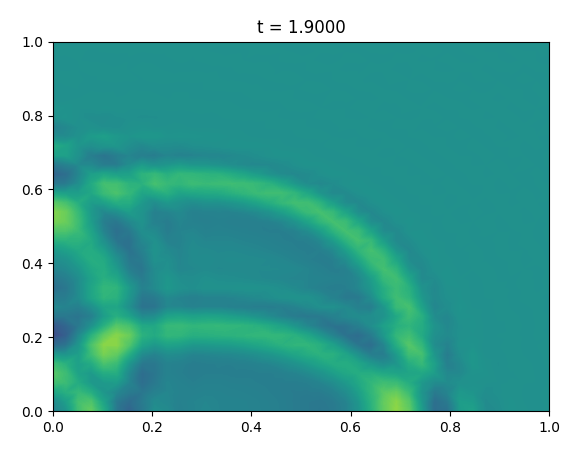
\includegraphics[width=0.5\textwidth]{figures/wave_eqn_outframe.png}
    \caption{Output of (\texttt{examples/demo\_wave\_equation.py}). A single frame of the wave equation demo code. The relevant solving code is provided in \autoref{fig:example-wave-timeloop}.}
    \label{fig:wave-eqn-frame}
\end{figure}
